\documentclass[journal,trans]{IEEEtran}

\usepackage[utf8]{inputenc}
\usepackage{graphicx}
\usepackage[spanish, es-tabla, activeacute]{babel}
\usepackage{verbatim}


\begin{document}

% Do not put math or special symbols in the title.
\newcommand{\titlepaper}{Diseño e Implementación de una ALU}

\title{\titlepaper}

\renewcommand\IEEEkeywordsname{Palabras clave}

\author{\IEEEauthorblockN{Adrián Dittel-Retana, Gabriel O. González-Rodríguez, Emmanuel Naranjo-Blanco, Jose Fabio Navarro-Naranjo, David Rodríguez-Camacho}

\IEEEauthorblockA{adriandittel19@estudiantec.cr}
\IEEEauthorblockA{gabrielgr01@estudiantec.cr}
\IEEEauthorblockA{naranjo760emm@estudiantec.cr}
\IEEEauthorblockA{josefabio1127@estudiantec.cr}
\IEEEauthorblockA{davo4006@estudiantec.cr}
\IEEEauthorblockA{\\Área Académica de Ingeniería Mecatrónica}
\IEEEauthorblockA{\\Instituto Tecnológico de Costa Rica}
}

% The paper headers
\markboth{Dittel, González, Naranjo, Navarro, Rodríguez, \titlepaper}%
{Shell \MakeLowercase{\textit{et al.}}: Bare Demo of IEEEtran.cls for Journals}

\IEEEtitleabstractindextext{%
\begin{abstract}
La Unidad Aritmética Lógica (ALU) consiste en una parte esencial de la unidad central de procesamiento, encargada de realizar operaciones lógicas y aritméticas para cumplir instrucciones dentro de un sistema computacional. En el presente proyecto de laboratorio se presentará una propuesta para el diseño de una ALU que lleva a cabo siete operaciones (lógicas y matemáticas), además de los resultados obtenidos tras su ejecución. La solución a la propuesta se basó fundamentalmente en el uso de lógica combinacional, y a nivel de diseño se utilizó el método de diseño modular, en donde se divide el sistema en subsistemas más pequeños, llamados módulos, a los cuales se les encuentra una solución individual, y reutilizable.  Posteriormente se integran las soluciones para cada módulo y se le agregan las distintas banderas como parte de las restricciones del proyecto. Una vez finalizado el experimento, se llega a la conclusión principal del proyecto: Se verificó mediante el lenguaje de descripción de hardware (HDL), y su implementación en la placa de desarrollo BASYS 3, el correcto funcionamiento de la ALU propuesta mediante la estructura de diseño planteada. Además, de la simulación se obtuvo, para la FPGA utilizada, un bajo consumo de potencia (5.576W) y una utilización del LUT (Look Up Table) de 0.33\%, lo que significa que también hubo un bajo consumo de memoria.
\end{abstract}

\begin{IEEEkeywords}
Diseño modular, ALU, Lógica Combinacional, Verilog.
\end{IEEEkeywords}}

\maketitle
\IEEEdisplaynontitleabstractindextext
\IEEEpeerreviewmaketitle

\section{INTRODUCCIÓN}

Parte fundamental de la electrónica digital consiste en la implementación de los conocimientos en la integración de sistemas completamente funcionales y aplicables para solucionar problemas de la vida real. En el presente proyecto de laboratorio se pretende aplicar la teoría, específicamente aquella relacionada con lógica combinacional, para así emplearla de forma práctica en una Unidad Aritmética Lógica (ALU, por sus siglas en inglés). 

De acuerdo con Tocci, una ALU consiste en un circuito que permite realizar operaciones lógicas y aritméticas \cite{Tocci}. Las cuales se encuentran como parte fundamental de los sistemas tecnológicos actuales como computadoras, celulares y tablets. A su vez, existen presentaciones en circuitos integrados como los chips 74LS382 o 74HC382 cuyo bloque se representa en la Figura \ref{fig:ALU}. 

En este tipo de chips se basa el objetivo específico del proyecto, el cual consiste en implementar un sistema lógico en un ambiente de verificación de hardware. Donde como parte de los objetivos generales se tiene comprender el proceso de diseño y verificación de los sistemas digitales, y aplicar el diseño en una placa de desarrollo. Para este caso se utiliza una matriz de puertas lógicas programable en campo, comúnmente llamada FPGA (Field-Programmable Gate Array).

\begin{figure}[!h]
	\centering
	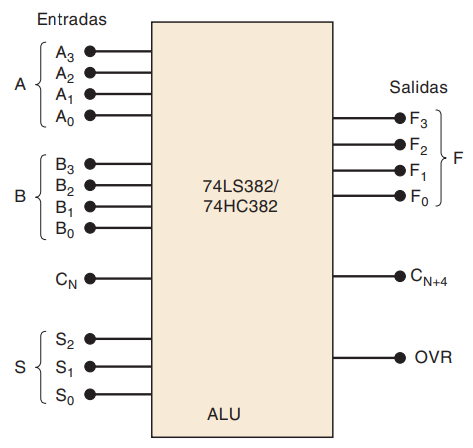
\includegraphics[width =0.7 \columnwidth]{Imagenes/ALU}
	\caption{Símbolo de bloque para el chip ALU 74LS382/HC382 \cite{Tocci}.}
	\label{fig:ALU}
\end{figure}

La idea fundamental de este proyecto consiste en diseñar una ALU que realice todas las operaciones descritas en la Tabla \ref{tab:operaciones}. Para esto se tienen dos entradas de datos A y B, y una salida Y, todas con un tamaño constante de palabra de 6 bits y operando bajo el sistema de complemento a dos. Además, las operaciones se escogen mediante un selector SEL de 3 bits y se requiere de tres banderas: cero, paridad par y desbordamiento. 

\begin{table}[!h]
  \begin{center}
    \caption{Descripción de las operaciones de la ALU por diseñar.}
    \label{tab:operaciones}
    \begin{tabular}{c | c | c }
      \hline
      SEL [2:0] & Tipo de Operación & Y \\
      \hline
       000 & XOR & Y = A $\string^$ B \\
       \hline
       001 & AND & Y = A $\&$ B \\
       \hline
       010 & OR & Y = A $\mid$ B \\
       \hline
       011 & Desplazamiento lógico a la derecha & Y=A $\gg$ 1 \\
       \hline
       100 & Suma con signo & Y = A + B \\
       \hline
       101 & Multiplicación con signo & Y = A * B \\
       \hline
       110 & Resta con signo & Y = A - B \\
       \hline
       111 & Quintuplicado de un número & Y = 5 * A \\
      \hline
    \end{tabular}
  \end{center}
\end{table}

Para simular e implementar el diseño propuesto se utiliza la placa BASYS 3 Artix-7 (xc7a35tcpg236-2L), la cual se programa en Verilog, un lenguaje de descripción de hardware (HDL, por sus siglas en inglés) al cual se le realiza una previa simulación para comprobar su correcto funcionamiento.

A modo conceptual, un HDL se trata de un lenguaje de programación para modelar un bloque de hardware, el cual permite simular la operación del circuito antes de fabricarlo \cite{Paulino}. En este caso, se trabajó con el HDL Verilog debido a su popularidad y simplicidad, y por ser estándar en la industria de las FPGA. Para esto, cada componente se describe con módulos y la verificación de este se establece bajo la estructura de un TestBench.

En las siguientes secciones se detallará el proceso de diseño junto con los diagramas modulares realizados y su descripción. Posteriormente se analizarán los resultados obtenidos tanto a nivel físico como simulado mediante el software Vivado. 


\section{DISEÑO DE LA ALU}

Para el desarrollo de la ALU anteriormente descrita, se utilizó un diseño modular, desarrollado y ejemplificado a través de diagramas de primer, segundo y tercer nivel (ver anexos).

Las restricciones previamente definidas para el proyecto son las siguiente:
\begin{itemize}
    \item Implementar todas las operaciones presentes en la tabla \ref{tab:operaciones}.
    \item Para las entradas de datos, debe permitir dos operandos (A y B) con un tamaño de palabra de 6 bits cada una y un selector (SEL) de 3 bits.
    \item Para la salida de datos, el resultado (Y) debe de tener también un tamaño de palabra de 6 bits.
    \item La ALU debe operar bajo el sistema complemento a 2.
    \item Deben implementarse 3 banderas de salida: cero (ZF), paridad par (PZ) y desbordamiento (OF).
\end{itemize}

Tomando en cuenta lo anterior, a continuación se presenta el diseño realizado clasificado en las tres etapas del diseño modular (primero, segundo y tercer nivel).


\subsection{PRIMER NIVEL}
En la figura \ref{fig:diagrama_1nivel} se muestra el diagrama de primer nivel formado a partir de las restricciones del proyecto. En dicha imagen se observan las 3 entradas presentes para el sistema (A y B números de 6 bits cada uno, y SEL de 3 bits), y las 4 salidas esperadas (Y de 6 bits, que es el resultado de la operación, y las 3 banderas de un bit cada una).

\begin{figure}[!h]
	\centering
	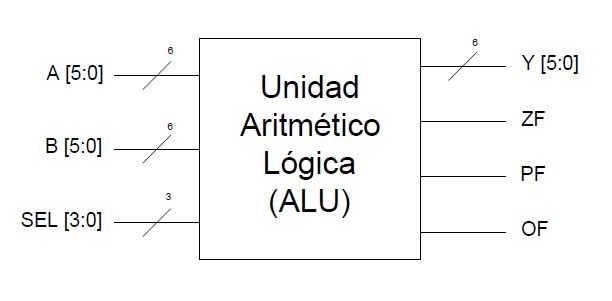
\includegraphics[width=0.8 \columnwidth]{Imagenes/diagrama_1nivel}
	\caption{ALU: Diagrama de primer nivel.}
	\label{fig:diagrama_1nivel}
\end{figure}


\subsection{SEGUNDO NIVEL}
En esta sección se decidió asignarle un módulo a cada operación descrita en la tabla \ref{tab:operaciones}, con excepción de las operaciones de suma y resta, que se unieron en un mismo módulo, esto debio a la gran similitud en los circuitos necesarios para realizar estas operaciones. Luego, se juntan por medio de un grupo de multiplexores 8 a 1 (un multiplexor por cada bit), encargado de controlar cuál resultado de las operaciones se transmite a la salida del sistema como Y.

Cada uno de estos módulos tiene como entradas a A y a B (a excepción de la operación de desplazamiento y de quintuplicación, las cuales solo operan con el número definido como A), y como salida al resultado de la operación correspondiente (de 6 bits también). Además, las operaciones de Sumador y restador, Multiplicador y Quintuplicador, poseen una salida extra correspondiente a la bandera de OF, las cuales se toman como entradas en el módulo encargado de ejecutar la bandera OF del sistema. Es importante mencionar, que las operaciones lógicas no tienen una bandera OF, ya que este valor siempre es cero para ellas.

Para finalizar, se agregaron los dos módulos faltantes (para las banderas ZF y PF), los cuales tienen a Y como entrada.

En la Figura \ref{fig:Diagrama_segundo_nivel} de los anexos, se puede observar el diagrama correspondiente a esta sección.

\subsection{TERCER NIVEL}
A continuación se describe el diseño realizado para cada uno de los módulos propuestos en la sección anterior.

\subsubsection{Bandera ZF}
Para la bandera de cero, o la “Zero Flag”, se colocó una compuerta del tipo NOR que toma todos los bits de salida del resultado de las operaciones, de modo que (al ser una compuerta NOR) arroje un 1 únicamente cuando todos los bits de Y sean 0. Este diagrama se puede observar en la Figura \ref{fig:Diagrama_tercer_nivel_ZF} de los anexos.

\subsubsection{Bandera PF}
Para la bandera de paridad par se utilizó una compuerta XNOR, la cual recibe como entrada todos los bits del resultado Y. Debido a su funcionamiento, provocará que la bandera se active (1 lógico) cuando la cantidad de bits iguales a 1 en la entrada sea par. Este diagrama se puede observar en la Figura \ref{fig:Diagrama_tercer_nivel_PF} de los anexos.

\subsubsection{Bandera OF}
Como se mencionó en la sección anterior, se toman todas las banderas de OF a la salida de las operaciones matemáticas y se utilizan como entrada para este módulo, que corresponde a un multiplexor 8 a 1, el cual usa el mismo selector del multiplexor que saca el bus de datos de las operaciones (es decir, el selector de las operaciones lógicas). De esta manera, se conecta la bandera OF del sistema a la salida de este multiplexor, y se refleja el desbordamiento de la operación que se está realizando. Es importante mencionar que las primeras 4 entradas del multiplexor son 0, ya que corresponden al desbordamiento de las operaciones lógicas. Este diagrama se puede observar en la Figura \ref{fig:Diagrama_tercer_nivel_OF} de los anexos. 

Por último, como se diseñó un único módulo para las operaciones de suma y resta, y como la bandera OF del módulo refleja el desbordamiento de la operación que se está realizando, las entradas 4 y 6 del multiplexor se encuentran en corto circuito con la bandera OF a la salida del circuito Sumador/Restador.

\subsubsection{XOR}
Para esta operación se implementó el uso de 6 compuertas XOR, las cuales comparan los bits de A contra los de B en el orden de significancia, es decir, la primera compuerta XOR compara el bit A0 con el bit B0, la segunda compuerta compara el bit A1 con el bit B1, y así sucesivamente. Este diagrama se puede observar en la Figura \ref{fig:Diagrama_tercer_nivel_xor} de los anexos. 

\subsubsection{AND}
El diseño para el circuito que ejecuta esta operación es bastante similar al implementado en la operación anterior, solo que con otro tipo de compuertas lógica. Utiliza 6 compuertas del tipo AND, las cuales comparan bit por bit, las entradas A y B, desde el bit menos significativo, hasta el bit más significativo, de modo que este circuito arroja como salida un bus de 6 bits, que incluye todas las salidas individuales de cada compuerta. Este diagrama se puede observar en la Figura \ref{fig:Diagrama_tercer_nivel_and} de los anexos. 

\subsubsection{OR}
De manera bastante similar a las anteriores, esta operación se realiza con 6 compuertas OR que comparaban uno a uno los bits de las entradas A y B, conforme a su significancia, de modo que al circuito le entran los 6 bits de A, y los 6 bits de B, y tiene como salida un bus de datos que se dirige al multiplexor, y que representa las salidas de cada compuerta OR individual. Este diagrama se puede observar en la Figura \ref{fig:Diagrama_tercer_nivel_or} de los anexos. 

\subsubsection{Desplazamiento lógico a la derecha}
Para el diseño de este circuito lógico, no se utilizó ninguna compuerta lógica. Lo que se realizó fue que se alambraron los bits de A, de modo que calzaran con el bit de Y esperado. Para esto, se utilizó de manera ilustrativa la Tabla 2, con el fin de tener una idea más clara de las conexiones a realizar. Este diagrama se puede observar en la Figura \ref{fig:Diagrama_tercer_nivel_desplazamiento} de los anexos.


\subsubsection{Sumador con signo y Restador con signo}
Para el diseño de estas operaciones se decidió implementarlas en un único circuito, el cual iba a seleccionar que operación realizar según el bit 1 del selector de la ALU (0 para suma y 1 para resta), se utilizó un sumador donde A se conecta directamente a una de sus entradas y B procede de la salida de un multiplexor (Mux) gobernado por SEL[1], en una entrada del Mux B se mantiene igual y en la otra se invierte con compuertas NOT. Igualmente, el acarreo de entrada corresponde a SEL[1]. De este modo, al escoger la suma, A y B se mantienen iguales y Cin = 0, pero al escoger la resta, A se mantiene y se aplica el complemento a 2 de B gracias a que este se niega a causa de la salida del Mux y se suma un 1 con el Cin = 1.

Para determinar si se tenía desbordamiento, se tomó en cuenta que, en la suma esta condición puede ocurrir solo cuando los operandos son del mismo signo y siempre produce un resultado incorrecto. Por otro lado, en la resta el desbordamiento sucede cuando los números tienen signos diferentes, con esto, entonces, al trabajar bajo el sistema de complemento a 2, se sabe que tanto para resta como para suma, si el número es negativo, se realizará el complemento a 2 de este y se hará la operación de suma. Por esta razón, el desbordamiento ocurre únicamente cuando el bit más significativo de los operandos es igual y el bit más significativo del resultado es distinto al MSB de los operandos. Este diagrama se puede observar en la Figura \ref{fig:Diagrama_tercer_nivel_suma_resta} de los anexos.

\subsubsection{Multiplicador con signo}
Para el diseño del multiplicador se utilizó el mismo algoritmo que se utilizaría para resolver una multiplicación binaria en complemento a dos a mano. Primero, se hace la conversión de complemento a 2 a binario natural para los operandos que tengan signo negativo. Segundo, se realiza la multiplicación binaria habitual con ambos operandos en binario natural. Y tercero, se hace una comprobación, por “ley de signos”, para determinar si el resultado debe de tener signo negativo o positivo.

Se hizo un módulo para el conversor de complemento a 2 / binario natural, en el cual se invierte cada bit del dato y luego se le suma uno. Este algoritmo funciona para hacer la conversión en cualquiera de las dos direcciones. Luego, mediante un multiplexor 2 a 1 se elije si transmitir el dato original o su conversión al módulo de multiplicación. La elección se realiza a partir del bit más significativo del dato, que se toma como selector. Al corresponder este al signo, si es positivo (0 lógico) se transmite el dato original y si es negativo (1 lógico) se transmite al conversión.

Se realiza lo anterior para ambos operandos y se procede a realizar la multiplicación en binario natural. Este módulo se construyó a partir de sumadores. El diagrama de este submódulo se puede observar en la figura \ref{fig:Diagrama_tercer_nivel_multiplicadorBinNat} de los anexos.

Por último, con otro multiplexor 2 a 1, se decide si transmitir como resultado del multiplicador el resultado de la multiplicación o su complemento a 2. Para realizar esta elección se toman el bit más significativo de cada operando como entrada de una compuerta XOR, y la salida se conecta al selector. De esta forma si el signo de los operandos es diferente, se transmite el complemento a 2 (resultado negativo), y si es igual, se transmite el resultado sin convertir (resultado positivo). 

El diagrama del multiplicador con signo se puede observar en la Figura \ref{fig:Diagrama_tercer_nivel_multiplicacion} de los anexos.

\subsubsection{Quintuplicador con signo}

En cuanto a la operación del quintuplicador, se hizo la multiplicación por 5 a partir del principio de desplazamiento a la izquierda. Dado que esto solo sirve para multiplicar por números resultantes de \((2^n)\), se separó el cinco en una suma de potencias de 2, \((2^2+2^0)\), entonces se corre el número entrante dos veces a la izquierda y se suma a la entrada original para obtener la función \(x(2^2+2^0)\).

Para esto se utilizó un circuito de dezplazamiento lógico a la izquierda que corre solo un bit entonces se conectan los 6 bits de entrada a este circuito y el resultado de este se vuelve a pasar por el circuito para obtener la multiplicación \((x*2^2)\) y esto es equivalente a multiplicar por 4 y a desplazar el número dos veces, por último este resultado y el número de entrada (sin cambios) del quintuplicador se suman para obtener el valor final de la multiplicación por cinco. 

Se creó un circuito para el desplazador (ver Figura \ref{fig:detalle_quintuplicador} de los anexos: detalle quintuplicador). El cuál es una colección de compuertas AND, OR y un bit de control. Cuando el bit de control es 0 el desplazador va a añadir un cero en la posición del bit menos significativo y las posiciones actuales de los otros bits restantes se cambian por los valores del bit anterior.

\section{IMPLEMENTACIÓN Y ANÁLISIS DE RESULTADOS}

Para realizar la implementación del diseño planteado anteriormente, se conectó la FPGA, para cargar el código generado en Verilog, esto a través de la máquina virtual, con esto entonces, se tomó la decisión de hacer la introducción de datos con los switches, tomando los iniciales del lado derecho y moviendose hacia la izquierda, siendo los primeros 3 switches, los 3 bits del seleccionador, luego los siguientes 6 switches para los bits de la entrada A y luego de la misma forma 6 switches para los 6 bits de B, esto respetando que siempre se inicia con el LSB con el switch más a la derecha; para determinar que valor se obtuvo en la salida Y, se decidió configurar los LEDs iniciando nuevamente a la derecha con el LSB moviendose hacia la izquierda, representando el valor de cada bit de Y, encendido si es 1, y apagado si es 0.

Una vez hecho esto, se hizo un análisis post-implementación para determinar que porcentajes de energía y de área fueron utilizados en el diseño, esto se puede observar en la figura \ref{fig:Resultados}.

\begin{figure}[!h]
	\centering
	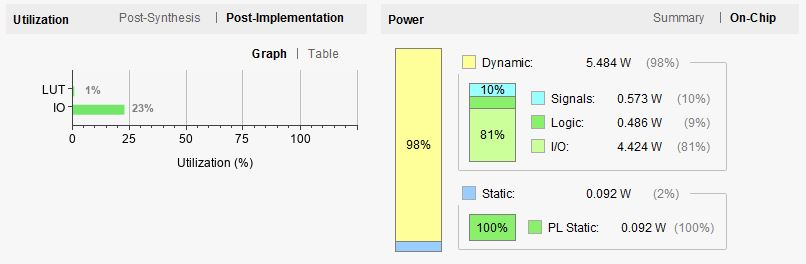
\includegraphics[width= \columnwidth]{Imagenes/Resultados}
	\caption{Resultados post-implementación de energía y área.}
	\label{fig:Resultados}
\end{figure}

Al observar  los datos obtenidos presentados anteriormente, se tiene que se obtuvo un sistema bastante eficiente en términos de espacio, como se presenta en la tabla \ref{tab:porcentajes}, y también de energía.

\begin{table}[!h]
  \begin{center}
    \caption{Porcentajes de utilización.}
    \label{tab:porcentajes}
    \begin{tabular}{c | c | c | c }
      \hline
      Recurso & Utilización & Disponible & Utilización (Porcentual\\
      \hline
       LUT & 68 & 20800 & 0.33 \\
    \end{tabular}
  \end{center}
\end{table}

En el aspecto de área de memoria utlizada, se tiene que, con un 0.33\% de la memoria total, el recurso utilizado es poco en comparación a todo el disponible, como se observa en la tabla \ref{tab:porcentajes}. Siendo este valor ni siquiera el 1\%, se puede concluir que el diseño planteado es de alta eficiencia, ya que al utilizar tan poco espacio permite que la FPGA, pueda llevar a cabo todas las operaciones planteadas de forma cómoda y sin problemas.

Por el otro lado, al analizar cuánta energía fue utilizada por la placa, se tiene que esta consumió una potencia de 5.576W, siendo 4.424W de los inputs y outputs del sistema y 0.486W de la lógica combinacional implementada en el diseño, como se ve en la figura \ref{fig:Resultados}. Por lo que, de toda la potencia utlizada, sólo el 9\% es dedicada a la lógica. Con todo lo anterior, se determina que el diseño planteado así como su construcción son sumamente eficientes en ambos aspectos evaluados.

\section{CONCLUSIONES}
A partir de este presente trabajo, se logró concluir lo siguiente.
\begin{itemize}
    \item El diseño propuesto realiza todas las operaciones lógicas y aritmeticas implementadas de forma correcta.
    \item El diseño propuesto obtuvo un bajo consumo de potencia (5.576W) para la FPGA BASYS 3 Artix-7.
    \item El diseño propuesto obtuvo un bajo consumo de memoria, 0.33\% del LUT, para la FPGA BASYS 3 Artix-7.
    \item Se obutvo el comportamiento esperado al realizar la implementación en la FPGA BASYS 3 Artix-7. Comprobando así la correctitud de las operaciones lógicas y aritméticas implementadas.
\end{itemize}


\section{RECOMENDACIONES}
Para realizar exitosamente el proyecto es necesario cumplir una serie de recomendaciones.
\begin{itemize}
    \item Es indispensable la partición del problema en subsistemas (diseño modular) por dos razones, para familiarizarse con los estándares de diseño y para comprender el proceso de solucionar sistemas digitales complejos que por medio de otras herramientas como tablas de verdad o funciones lógicas únicamente, no se podría, o se volvería innecesariamente complicado.
    \item La utilización de diseño modular facilita considerablemente la depuración en caso de cometer un error.
    \item Es de suma importancia que a la hora de crear los diseños se hagan con la simplificación al máximo ya que esto permite lograr bajos valores de consumo de energía y espacio.
    \item Para cada nuevo módulo que se cree en Verilog se debe de hacer su correspondiente TestBench para garantizar que el funcionamiento es el que se planteó, de igual forma, probarlo con la mayor cantidad de casos posibles.
\end{itemize}


\section{ANEXOS}
En esta sección se presentan los diversos diagramas de segundo y tercer nivel que representan todos los aspectos del diseño propuesto. Se incluyen el diagrama general de la solución y los diagramas para todas las operaciones (tanto lógicas como matemáticas) así como para las banderas solicitadas.

\begin{figure}[h!]
	\centering
	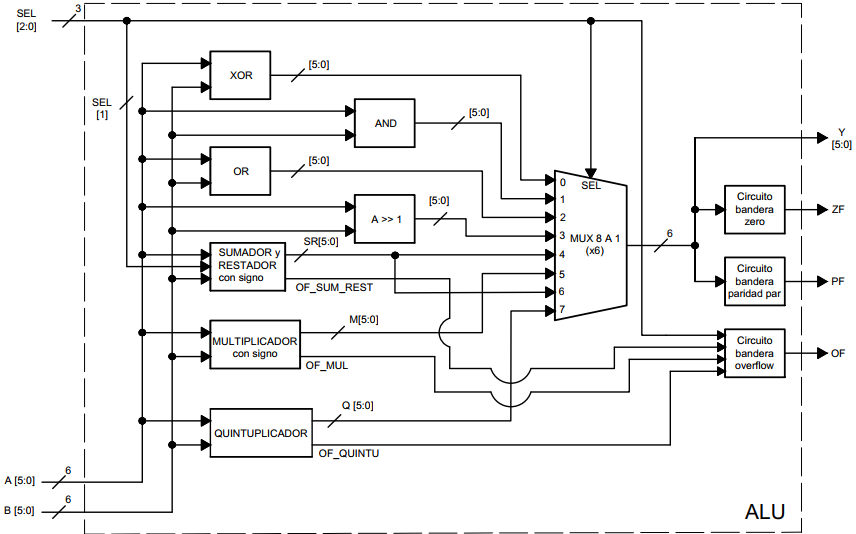
\includegraphics[width=1 \columnwidth]{Imagenes/Diagrama_segundo_nivel.png}
	\caption{ALU: Diagrama de segundo nivel.}
	\label{fig:Diagrama_segundo_nivel}
\end{figure}

\begin{figure}[h!]
	\centering
	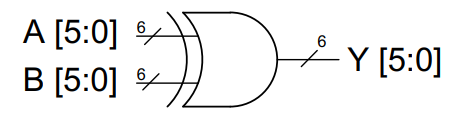
\includegraphics[width=0.5 \columnwidth]{Imagenes/Diagrama_tercer_nivel_xor.png}
	\caption{ALU: Diagrama de tercer nivel de la operación XOR.}
	\label{fig:Diagrama_tercer_nivel_xor}
\end{figure}

\begin{figure}[h!]
	\centering
	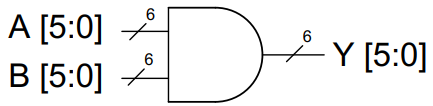
\includegraphics[width=0.5 \columnwidth]{Imagenes/Diagrama_tercer_nivel_and.png}
	\caption{ALU: Diagrama de tercer nivel de la operación AND.}
	\label{fig:Diagrama_tercer_nivel_and}
\end{figure}

\begin{figure}[h!]
	\centering
	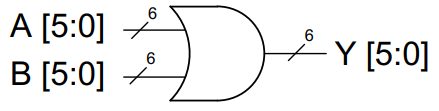
\includegraphics[width=0.5 \columnwidth]{Imagenes/Diagrama_tercer_nivel_or.png}
	\caption{ALU: Diagrama de tercer nivel de la operación OR.}
	\label{fig:Diagrama_tercer_nivel_or}
\end{figure}

\begin{figure}[h!]
	\centering
	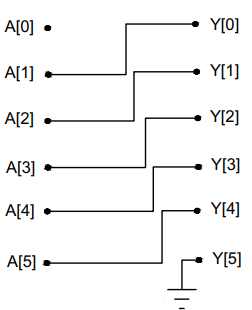
\includegraphics[width=0.5 \columnwidth]{Imagenes/Diagrama_tercer_nivel_desplazamiento.png}
	\caption{ALU: Diagrama de tercer nivel de la operación desplazamiento lógico a la derecha.}
	\label{fig:Diagrama_tercer_nivel_desplazamiento}
\end{figure}

\begin{figure}[h!]
	\centering
	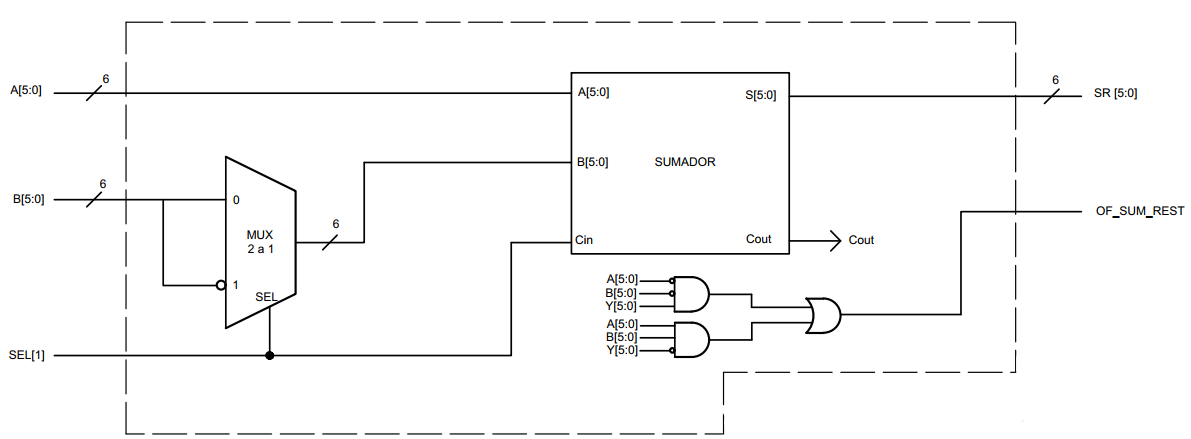
\includegraphics[width=1 \columnwidth]{Imagenes/Diagrama_tercer_nivel_suma_resta.png}
	\caption{ALU: Diagrama de tercer nivel de las operaciones de suma y resta con signo.}
	\label{fig:Diagrama_tercer_nivel_suma_resta}
\end{figure}

\begin{figure}[h!]
	\centering
	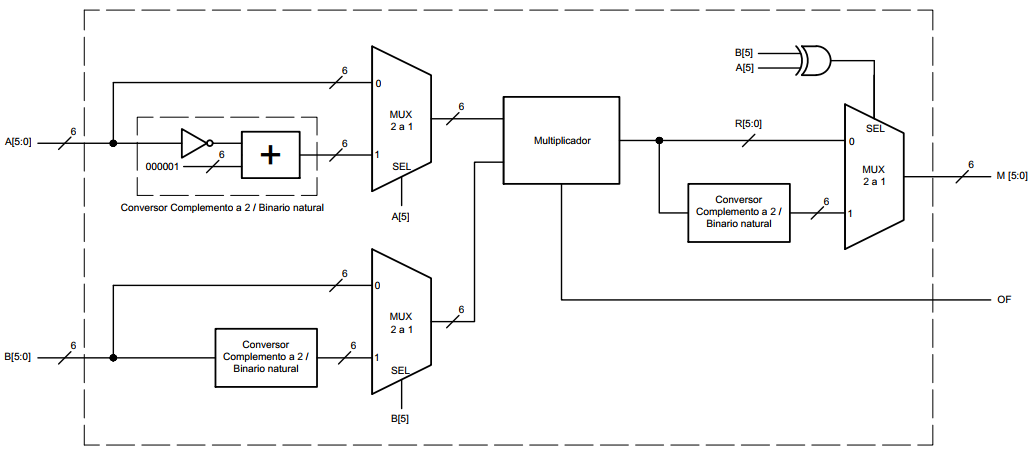
\includegraphics[width=1 \columnwidth]{Imagenes/Diagrama_tercer_nivel_multiplicacion.png}
	\caption{ALU: Diagrama de tercer nivel de la operación de multiplicación con signo.}
	\label{fig:Diagrama_tercer_nivel_multiplicacion}
\end{figure}

\begin{figure}[h!]
	\centering
	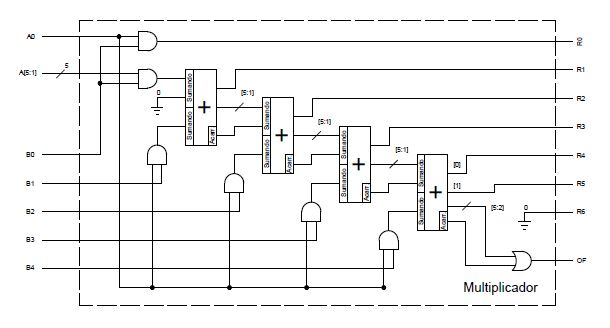
\includegraphics[width=1 \columnwidth]{Imagenes/Diagrama_tercer_nivel_multiplicadorBinNat.JPG}
	\caption{ALU: Diagrama de tercer nivel del submódulo correspondiente al multiplicador en binario natural.}
	\label{fig:Diagrama_tercer_nivel_multiplicadorBinNat}
\end{figure}

\begin{figure}[h!]
	\centering
	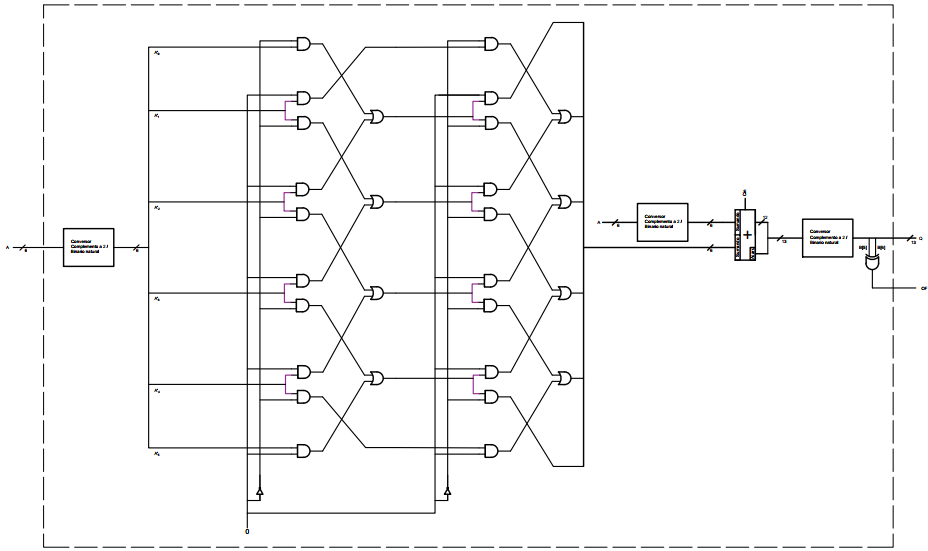
\includegraphics[width=1 \columnwidth]{Imagenes/Diagrama_tercer_nivel_quintuplicacion.png}
	\caption{ALU: Diagrama de tercer nivel de la operación de quintuplicado de un número.}
	\label{fig:Diagrama_tercer_nivel_quintuplicacion}
\end{figure}

\begin{figure}[h!]
	\centering
	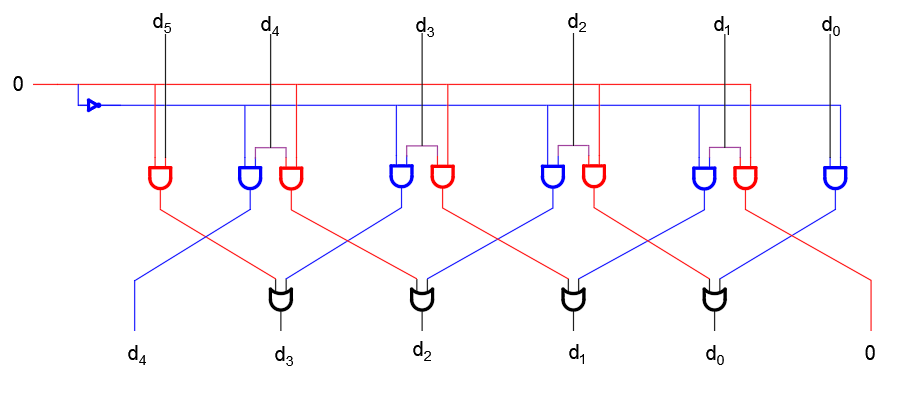
\includegraphics[width=1 \columnwidth]{Imagenes/detalle_quintuplicador.png}
	\caption{ALU: Detalle del circuito quintuplicador de un número.}
	\label{fig:detalle_quintuplicador}
\end{figure}

\begin{figure}[h!]
	\centering
	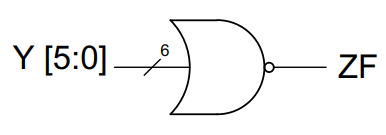
\includegraphics[width=0.6 \columnwidth]{Imagenes/Diagrama_tercer_nivel_ZF.png}
	\caption{ALU: Diagrama de tercer nivel para la bandera ZF.}
	\label{fig:Diagrama_tercer_nivel_ZF}
\end{figure}

\begin{figure}[h!]
	\centering
	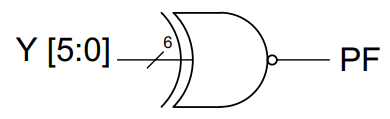
\includegraphics[width=0.6 \columnwidth]{Imagenes/Diagrama_tercer_nivel_PF.png}
	\caption{ALU: Diagrama de tercer nivel para la bandera PF.}
	\label{fig:Diagrama_tercer_nivel_PF}
\end{figure}

\begin{figure}[h!]
	\centering
	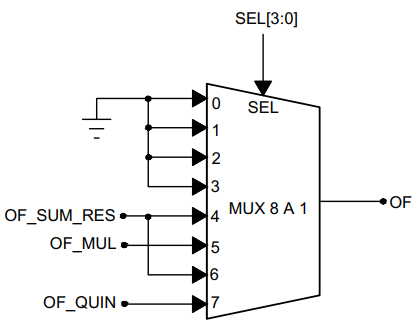
\includegraphics[width=0.7 \columnwidth]{Imagenes/Diagrama_tercer_nivel_OF.png}
	\caption{ALU: Diagrama de tercer nivel para la bandera OF.}
	\label{fig:Diagrama_tercer_nivel_OF}
\end{figure}

\newpage

\begin{thebibliography}{1}

\bibitem{Tocci}
R. Tocci. \emph{Sistemas digitales: Principios y aplicaciones}. Décima edición. Pearson Education. 2007.

\bibitem{Paulino}
Paulino Ruiz de Clavijo Vásquez. \emph{Introducción a HDL Verilog - Presentaciones de clase}. Departamento de Tecnología Electrónica. Universidad de Sevilla.


\end{thebibliography}

\end{document}
